\documentclass[main.tex]{subfiles}
\begin{document}

\chapter{Process Analysis}

\begin{figure}[h]
\centering
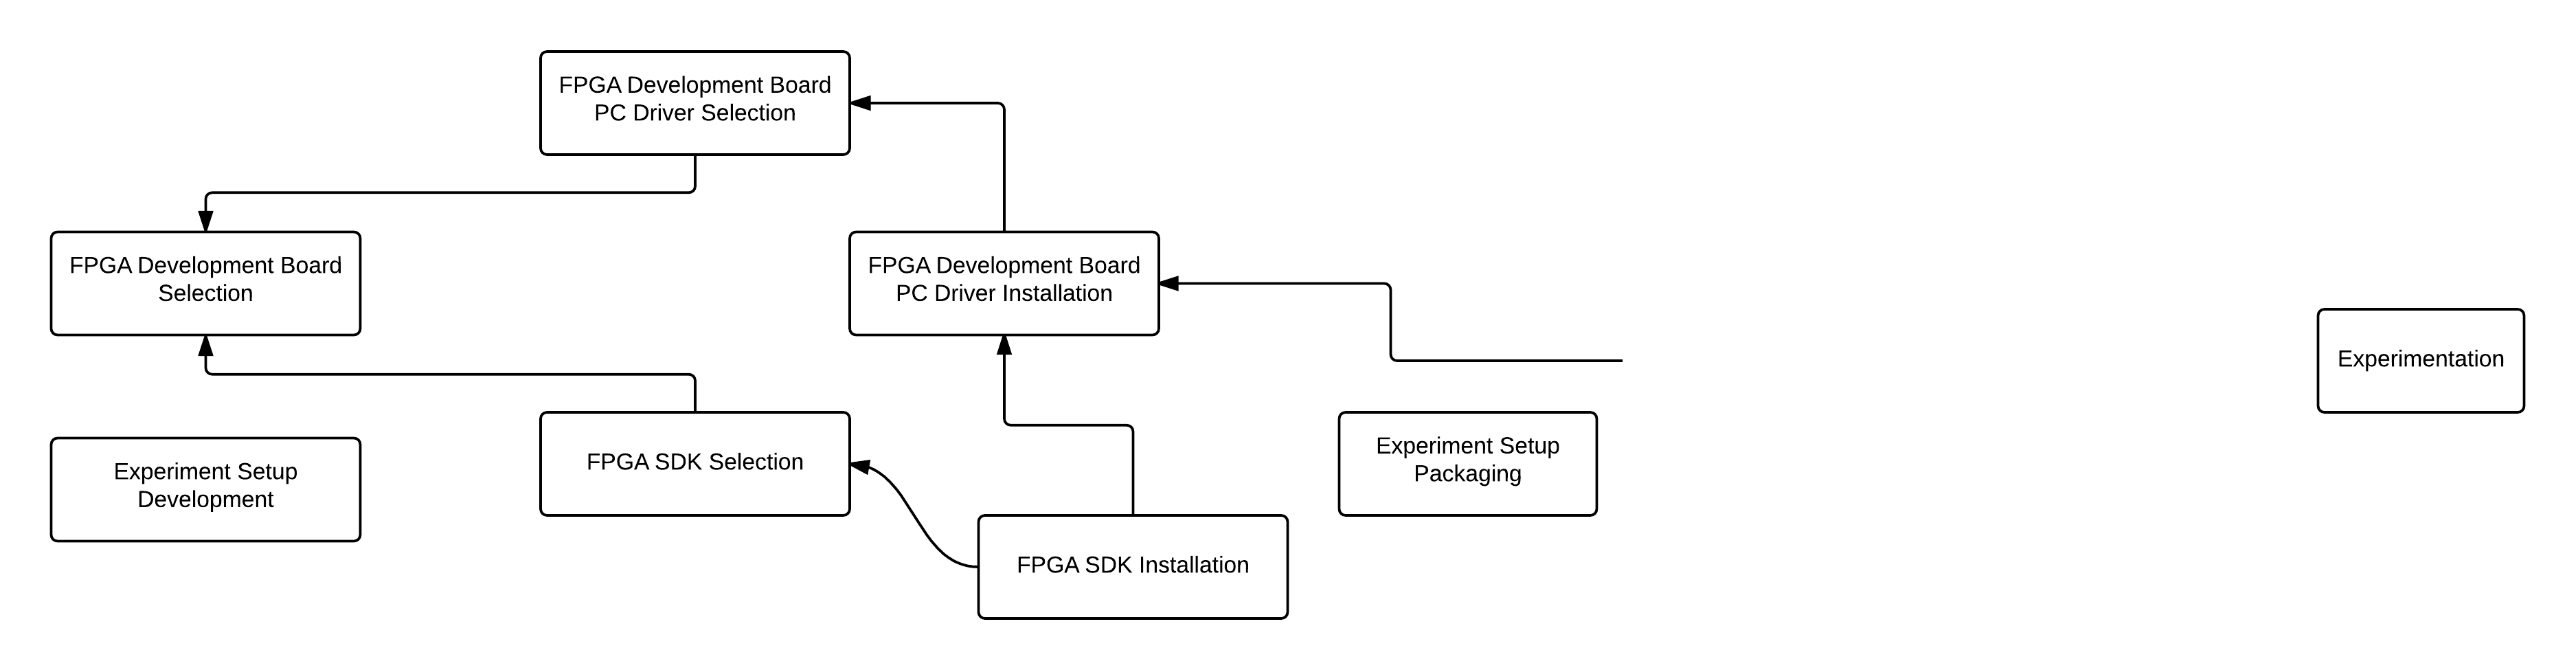
\includegraphics[width=\textwidth]{img/processes-dependencies-basic}
\caption{The basic model, process dependency graph}
\label{fig:dependencies-basic}
\end{figure}

\begin{figure}[h]
\centering
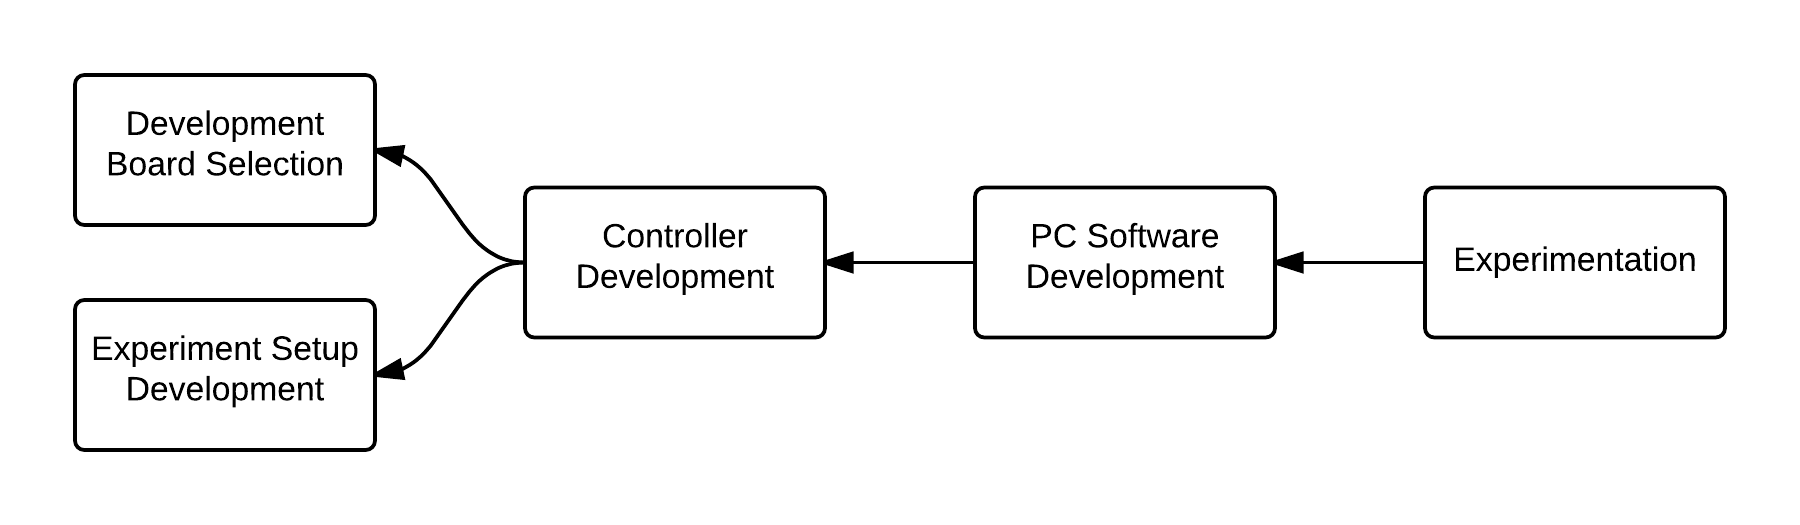
\includegraphics[width=\textwidth]{img/processes-dependencies-inout}
\caption{I/O virtualized, process dependency graph}
\label{fig:dependencies-inout}
\end{figure}

\begin{landscape}
\begin{figure}
\centering
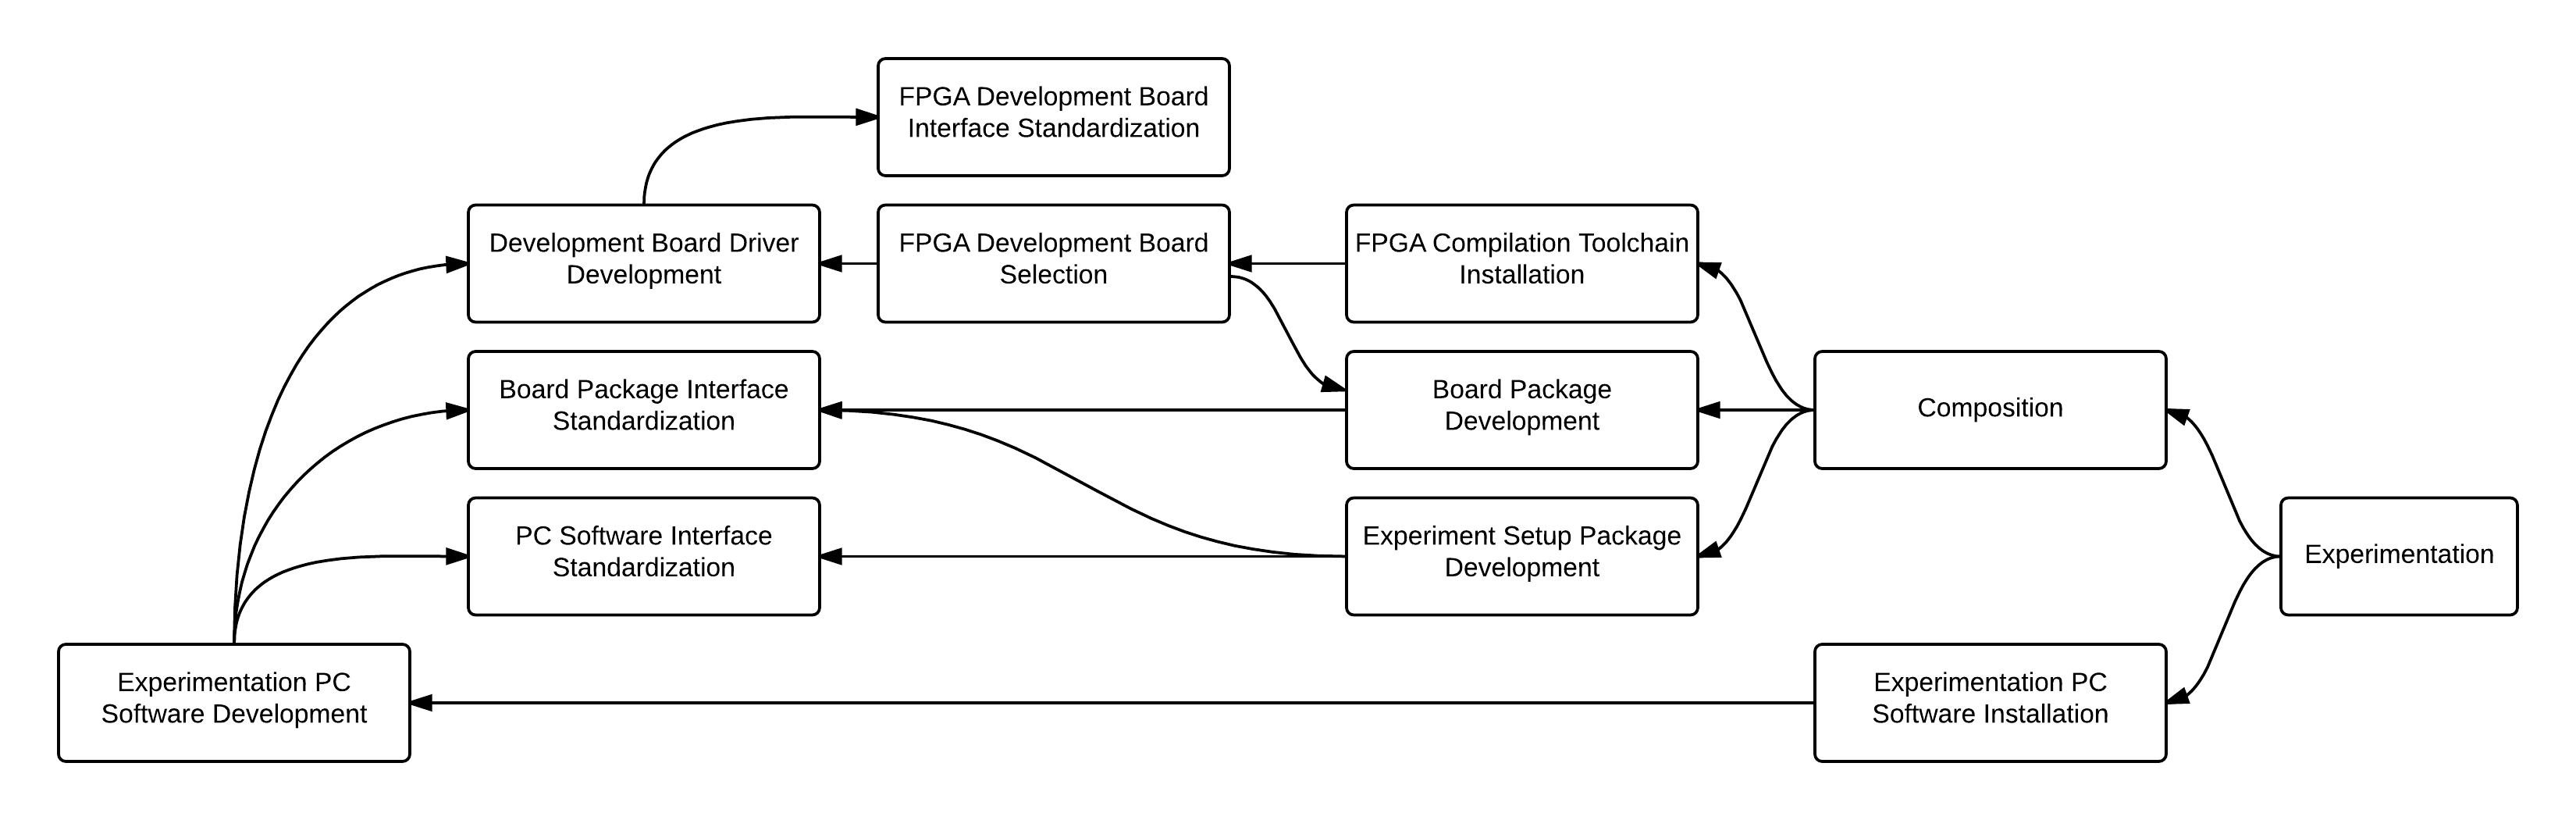
\includegraphics[width=\hsize]{img/processes-dependencies-control}
\caption{Cycle control, process dependency graph}
\label{fig:dependencies-control}
\end{figure}
\end{landscape}

\begin{landscape}
\begin{figure}
\centering
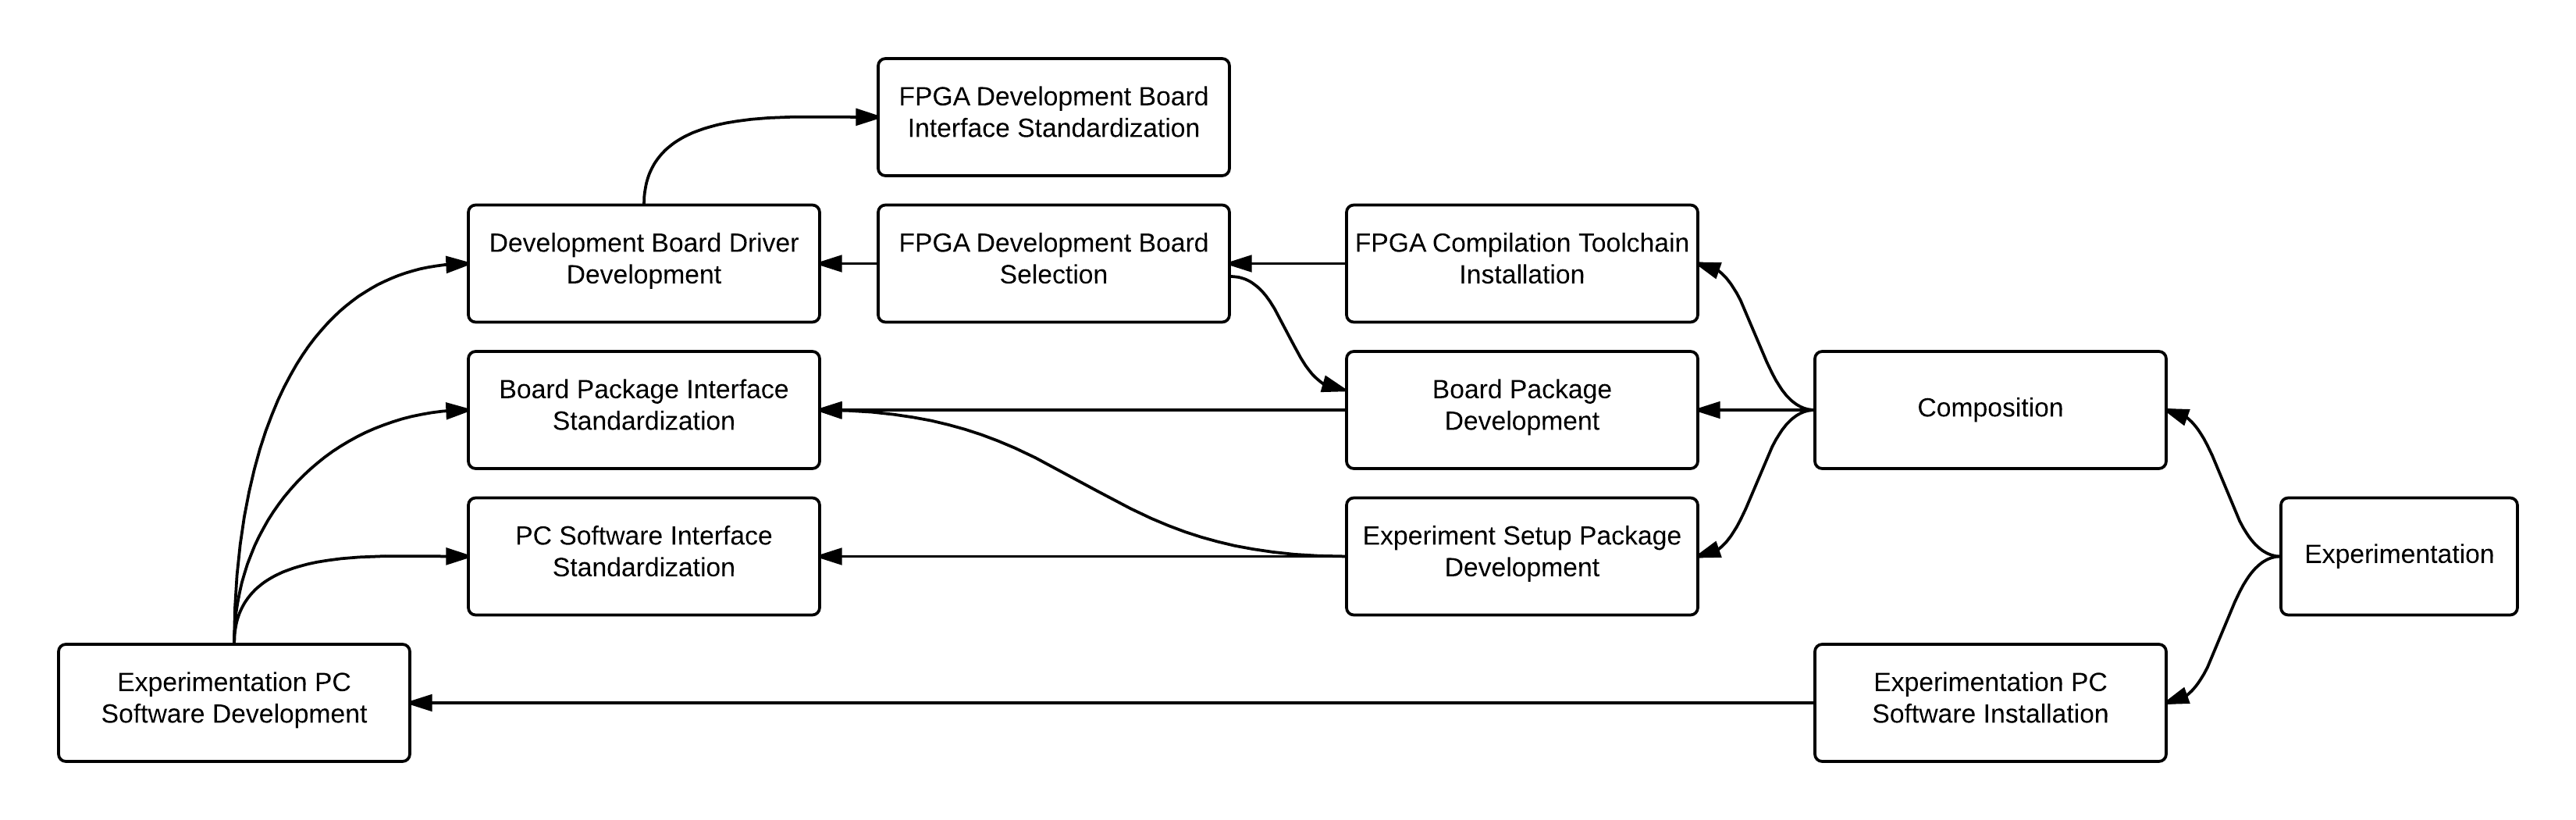
\includegraphics[width=\hsize]{img/processes-dependencies-abstract}
\caption{Controller abstracted, process dependency graph}
\label{fig:dependencies-abstract}
\end{figure}
\end{landscape}

\begin{landscape}
\begin{figure}
\centering
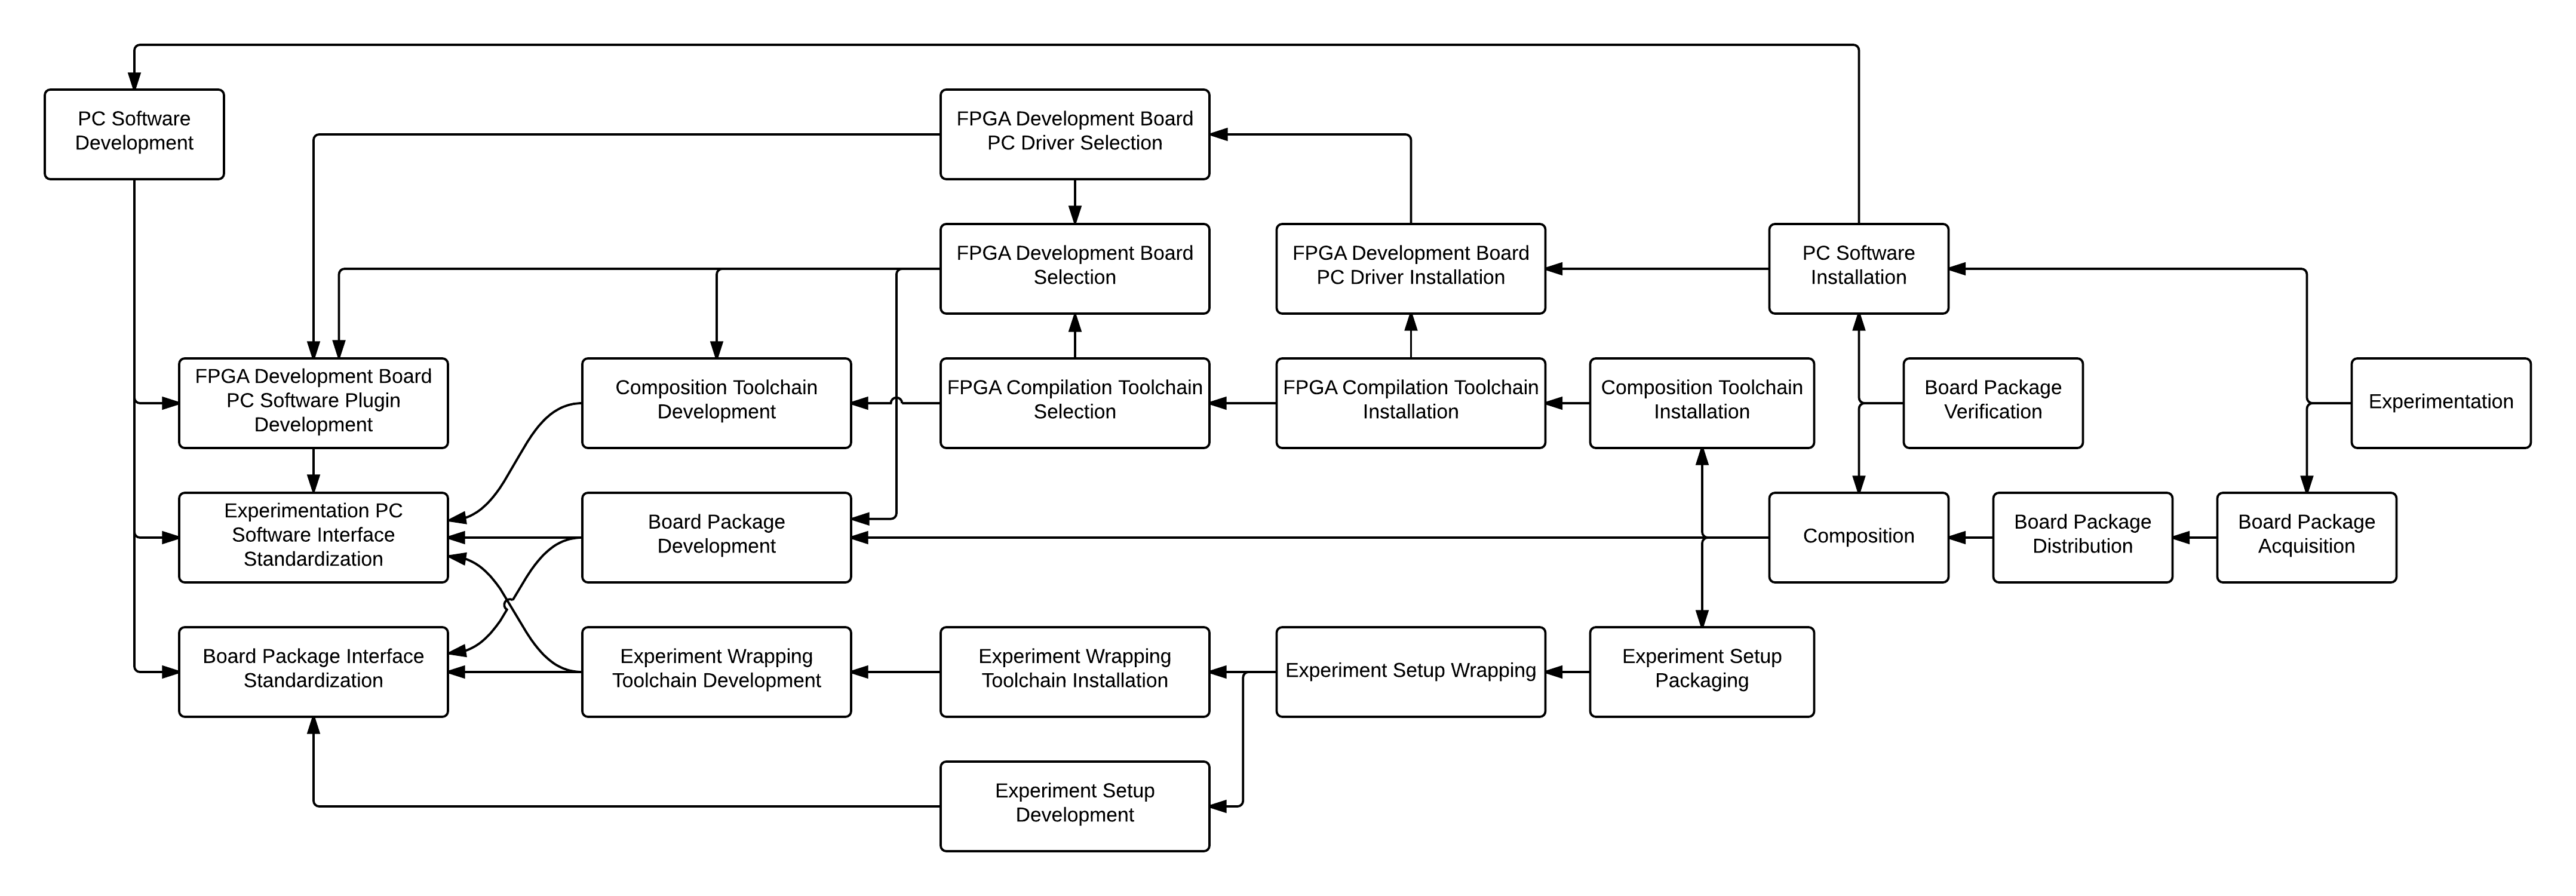
\includegraphics[width=\hsize]{img/processes-dependencies-io}
\caption{I/O reintroduced, process dependency graph}
\label{fig:dependencies-io}
\end{figure}
\end{landscape}

\end{document}